En este módulo se detalla la implementación de cada paso del preprocesamiento de los datos, también conocido como canalización del procesamiento de lenguaje natural. Este proceso comienza con la adquisición de los datos, detallada en el capítulo 3, que consiste en numerosos documentos de texto que deben ser tratados.


El preprocesamiento de texto incluye diversas tareas de limpieza necesarias para los archivos de comentarios adquiridos, así como la corrección de lenguaje requerida y la conversión y tratamiento de formatos de los archivos. Esto asegura su limpieza y utilidad para el entrenamiento de modelos y el manejo de numerosos archivos. El resultado es un conjunto de datos útil, limpio, bien distribuido y en uno de los formatos estándar aceptables para el entrenamiento de los modelos propuestos.


Dado que las tareas son numerosas, el módulo se dividió en secciones, cada una con un propósito específico, las cuales se describen a continuación:

Limpieza de Datos

La carpeta limpiezadataset almacena los siguientes archivos:


\begin{itemize}

\item limpiar\_datos.py: Este archivo se encarga de los aspectos específicos de limpieza para cada fuente de información. Por ejemplo, la limpieza de datos extraídos de la red social Facebook no será la misma que la de datos provenientes de la red social WhatsApp. Las funciones y detalles de este archivo se ilustran en la figura \ref{fig:uml1}.

\begin{figure}
	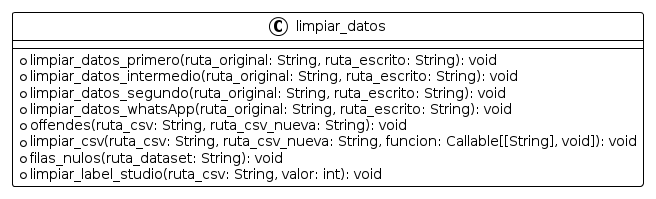
\includegraphics[width=0.65\textwidth]{capitulo5/figuras/fig1.png}
	\caption{Clase limpiar\_datos}
	\floatfoot{Fuente: Elaboración propia, generado con PlantUML}
	\label{fig:uml1}
\end{figure}

\item corrector\_lenguaje.py: Este archivo aborda los aspectos generales de limpieza que se aplican a cualquier tipo de información, independientemente de su fuente. Los detalles de este archivo se muestran en la figura \ref{fig:uml2}.

\begin{figure}
	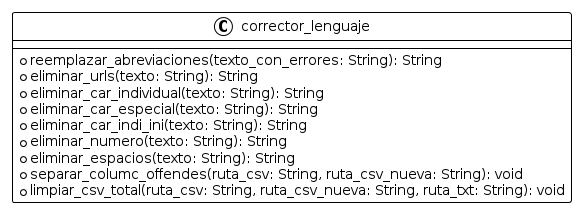
\includegraphics[width=0.65\textwidth]{capitulo5/figuras/fig2.png}
	\caption{Clase corrector\_lenguaje}
	\floatfoot{Fuente: Elaboración propia, generado con PlantUML}
	\label{fig:uml2}
\end{figure}

\end{itemize}

Formato y Encadenamiento de Información

La carpeta gestionarchivos contiene los siguientes archivos:

\begin{itemize}

\item manejo\_archivos.py: Este archivo se encarga de la creación, copia, recorrido y vaciado de archivos en diferentes formatos. Para más detalles, consulte la figura \ref{fig:uml3}.

\begin{figure}
	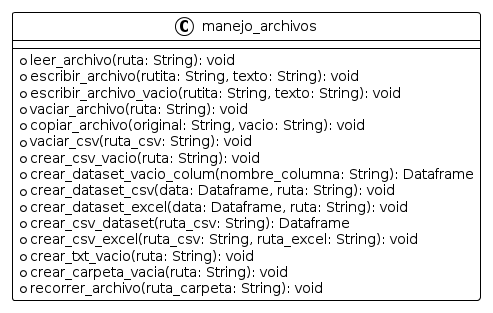
\includegraphics[width=0.65\textwidth]{capitulo5/figuras/fig3.png}
	\caption{Clase manejo\_archivos}
	\floatfoot{Fuente: Elaboración propia, generado con PlantUML}
	\label{fig:uml3}
\end{figure}


\item convertir\_formato.py: Este archivo se ocupa de agrupar información de múltiples archivos para hacer uso de forma masiva de las funciones de limpieza definidas en el archivo limpiar\_datos.py, además de manejar el formato de los mismos cuando sea necesario . Para más detalles, consulte la figura \ref{fig:uml4}.

\begin{figure}
	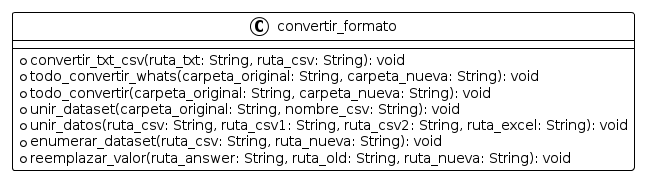
\includegraphics[width=0.65\textwidth]{capitulo5/figuras/fig4.png}
	\caption{Clase convertir\_formato}
	\floatfoot{Fuente: Elaboración propia, generado con PlantUML}
	\label{fig:uml4}
\end{figure}

\end{itemize}

Después de que los datos pasan por todo el proceso de canalización, se obtiene un producto final listo para ser utilizado en modelos de aprendizaje. Es importante recordar que el preprocesamiento de datos varía según la fuente de los datos. Para más detalles sobre el proceso de datos provenientes de Facebook, consulte la figura \ref{fig:um12} (diagrama de actividades de Facebook). El proceso de datos provenientes de WhatsApp se puede ver en la figura \ref{fig:um14}, y el proceso de limpieza del conjunto de datos ``offendes'' se detalla en la figura \ref{fig:um13}.

\begin{figure}
	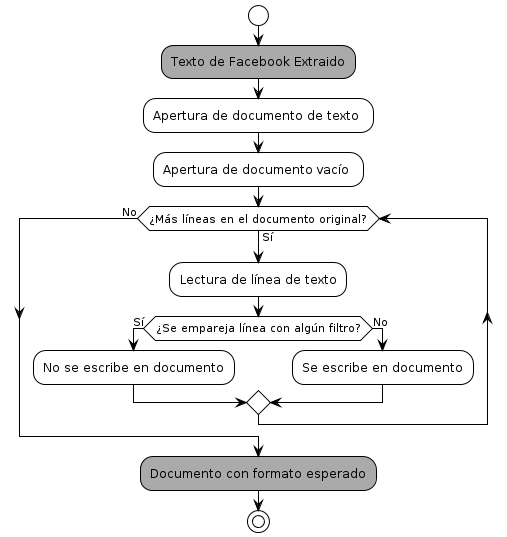
\includegraphics[width=0.65\textwidth]{capitulo5/figuras/part0.png}
	\caption{Diagrama de actividades limpieza datos facebook}
	\floatfoot{Fuente: Elaboración propia, generado con PlantUML}
	\label{fig:um12}
\end{figure}

\begin{figure}
	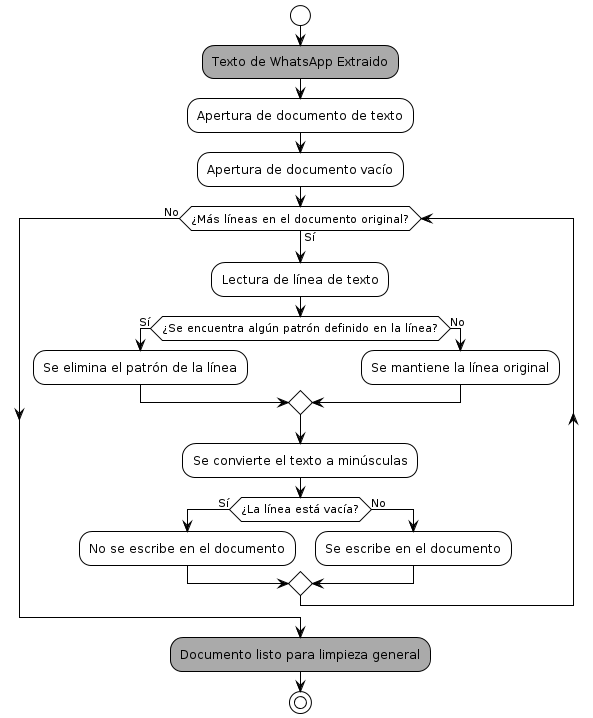
\includegraphics[width=0.65\textwidth]{capitulo5/figuras/part3.png}
	\caption{Diagrama de actividades limpieza datos whatsapp}
	\floatfoot{Fuente: Elaboración propia, generado con PlantUML}
	\label{fig:um14}
\end{figure}


\begin{figure}
	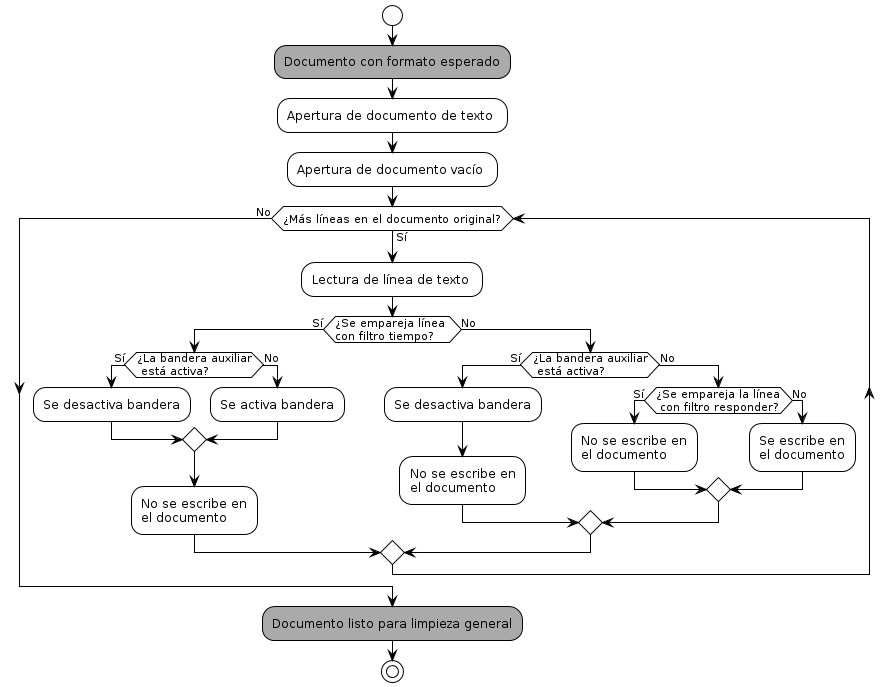
\includegraphics[width=0.65\textwidth]{capitulo5/figuras/part1.png}
	\caption{Diagrama de actividades  limpieza del conjunto de datos ``offendes''}
	\floatfoot{Fuente: Elaboración propia, generado con PlantUML}
	\label{fig:um13}
\end{figure}
